% -*- TeX -*- -*- UK -*- -*- Soft -*-

\chapter{Exploring Bayesian Theory}
\label{chap:ExploringBayesianTheory}



\section{Counting Balls}
\label{sec:CountingBalls}
\subsection{The Frequentist Way}
\label{sec:TheFrequentistWay}

McElreath \cite{McElreath2015} considers the problem of drawing coloured balls from a bag.  The bag is known to contain four balls, either white [W] or blue [B].  Three balls are drawn from the bag, the colour noted and the ball returned to the bag: on each draw there will be the same four balls in the bag.

Three balls are drawn as follows: [BWB]. What is the contents of the bag, how many white balls and how many blue balls?  There are five different conjectures and for each of these conjectures the number of ways to produce the draw is shown in the figure.
\begin{marginfigure}
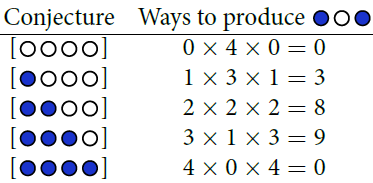
\includegraphics{p05c02-01}
\end{marginfigure}
The ways to produce the draw is found by multiplying for each conjecture the number of possible ways that each of the drawn balls could appear.  The draw produced blue and while balls, hence the first and the last conjecture are unable to produce the observed draw (0 ways). For each of the remaining conjectures the number of production ways are non-zero, reaching a maximum of nine, for the [BBBW] conjecture --- clearly this is the most plausible (but certainly not the only) bag contents.  At a much lower likelihood the [BWWW] bag contents could also produce the observed draw.
%By normalising ($n$/(0+3+8+9+0)) for the number of ways, the likelihood for the bag contents is
%[WWWW]=0\%, 
%[BWWW]=15\%,
%[BBWW]=40\%,
%[BBBW]=45\%, and
%[BBBB]=0\%.  These values represent the certainty we have for each of the conjectures.

\subsection{Using Prior Information}
\label{sec:UsingPriorInformation}

Using the results from the first three draws above, and we draw a fourth ball, what can we learn about the bags?  Suppose the fourth ball is blue [B].  Extend the previous calculation, and note how many ways a blue ball can be drawn.
\begin{marginfigure}
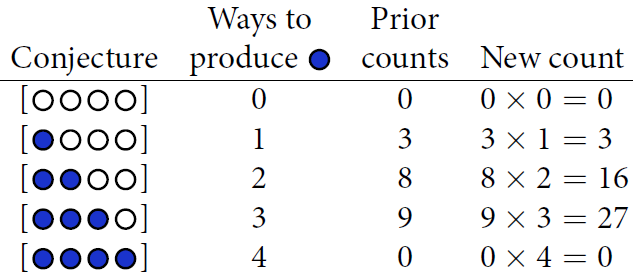
\includegraphics{p05c02-02}
\end{marginfigure}
Then multiply each of these new counts by the prior numbers of ways for each conjecture (the motivation for this follows below).  The diagram shows the bag contents likelihood if  drawing the following four balls:  [BWBB].
In this example the prior information is the first three balls drawn, the prior data and the new draw are of the same type (balls drawn).  Prior information may also arise from other sources, not just previous draws.

McElreath \cite{McElreath2015} continues his example by informing that 
someone from the marble factory tells you that blue marbles are rare. So for every bag containing [BBBW], they made two bags containing [BBWW] and three bags containing [BWWW]. They also ensured that every bag contained at least one blue and one white marble.
This prior information is multiplied with the counts after the four balls drawn thus far.
\begin{marginfigure}
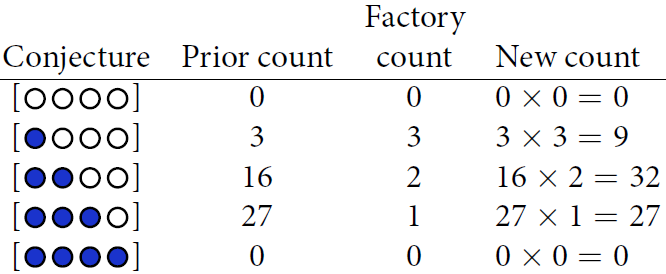
\includegraphics{p05c02-03}
\end{marginfigure}
%By normalising ($n$/(0+9+32+27+0)) for the number of ways, the likelihood for the bag contents, based on four draws and the factory prior information, is
%[WWWW]=0\%, 
%[BWWW]=13.2\%,
%[BBWW]=47.1\%,
%[BBBW]=39.7\%, and
%[BBBB]=0\%.  These values represent the certainty we have for each of the conjectures.

How is prior information obtained?  Prior information can be based on previous data (previous draws in this case), but more often on 'other' sources of information, such as a model of the process or the problem context. In the absence of prior information, unity values (a.k.a. \textit{flat priors}) can be assumed.  McElreath  calls this the \textit{Principle of Indifference} or \textit{Ignorance Priors}: When there is no reason to say that one conjecture is more plausible than another, weigh all of the conjectures equally. ``The principle of indifference results in inferences very comparable to mainstream non-Bayesian approaches [i.e., frequentist], most of which contain implicit equal weighting of possibilities. For example a typical non-Bayesian confidence interval weighs equally all of the possible values a parameter could take, regardless of how implausible some of them are.''\cite{McElreath2015}  Although McElreath ``does not endorse ignorance priors'' many problems use such ignorance or flat priors as starting values, and update these as the problem is developed or better understood.


